% !TEX root = ../../../main.tex
% 来源：中学数学实验教材·第三册（高中数学）
% 章节：直线、平面坐标化 / 直线坐标化
% 原始文件：2.tex，行 190-228
% 类型：tikz
% ---
    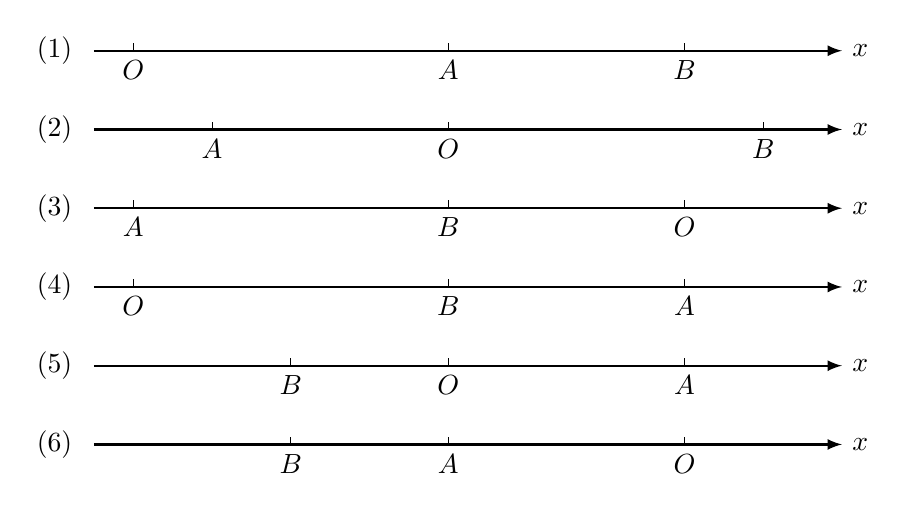
\begin{tikzpicture}[>=latex]
\foreach \y in {-1,-2,...,-6}
{
    \draw[->, thick](-4.5,\y)--(5,\y)node[right]{$x$};
}
\foreach \x/\xtext in {-4/O,0/A,3/B}
{
    \draw (\x,-1)--(\x,-1+.1);
    \node at (\x,-1)[below] {$\xtext$};
}
\foreach \x/\xtext in {-3/A,0/O,4/B}
{
    \draw (\x,-2)--(\x,-2+.1);
    \node at (\x,-2)[below] {$\xtext$};
}
\foreach \x/\xtext in {-4/A,0/B,3/O}
{
    \draw (\x,-3)--(\x,-3+.1);
    \node at (\x,-3)[below] {$\xtext$};
}
\foreach \x/\xtext in {-4/O,0/B,3/A}
{
    \draw (\x,-4)--(\x,-4+.1);
    \node at (\x,-4)[below] {$\xtext$};
}
\foreach \x/\xtext in {-2/B,0/O,3/A}
{
    \draw (\x,-5)--(\x,-5+.1);
    \node at (\x,-5)[below] {$\xtext$};
}
\foreach \x/\xtext in {-2/B,0/A,3/O}
{
    \draw (\x,-6)--(\x,-6+.1);
    \node at (\x,-6)[below] {$\xtext$};
}
\node at (-5,-1){(1)};\node at (-5,-2){(2)};
\node at (-5,-3){(3)};\node at (-5,-4){(4)};
\node at (-5,-5){(5)};\node at (-5,-6){(6)};
    \end{tikzpicture}
